\documentclass[twoside,11pt]{article}

% An Introduction to Visualisation Software for Astronomy.

% Copyright 1997  Starlink, CCLRC.

% This document is offered in good faith.  However, no guarantee or
% warranty whatsoever is offered or implied.  Neither myself, the
% University of Edinburgh nor the CCLRC accept any responsibility for
% loss, damage or injury resulting from the use of this document.

% A.C. Davenhall,
% 4th March 1997.

% ? Specify used packages
\usepackage{graphicx}        %  Use this one for final production.
% \usepackage[draft]{graphicx} %  Use this one for drafting.
% ? End of specify used packages

\pagestyle{myheadings}

% -----------------------------------------------------------------------------
% ? Document identification
\newcommand{\stardoccategory}  {Starlink Guide}
\newcommand{\stardocinitials}  {SG}
\newcommand{\stardocsource}    {sg\stardocnumber}
\newcommand{\stardocnumber}    {8.2}
\newcommand{\stardocauthors}   {A C Davenhall}
\newcommand{\stardocdate}      {4th March 1997}
\newcommand{\stardoctitle}     {An Introduction to \\ Visualisation
Software for Astronomy}
\newcommand{\stardocabstract}  {
This document is an introduction to various common visualisation
techniques and packages which might be used on Starlink systems. It is
aimed at astronomers with complex datasets to display and explore but
no prior knowledge of visualisation techniques. Its purpose is to
assist such an astronomer to find visualisation software suitable for his
problem. It is not a manual for any particular package.}

% ? End of document identification
% -----------------------------------------------------------------------------

\newcommand{\stardocname}{\stardocinitials /\stardocnumber}
\markboth{\stardocname}{\stardocname}
\setlength{\textwidth}{160mm}
\setlength{\textheight}{230mm}
\setlength{\topmargin}{-2mm}
\setlength{\oddsidemargin}{0mm}
\setlength{\evensidemargin}{0mm}
\setlength{\parindent}{0mm}
\setlength{\parskip}{\medskipamount}
\setlength{\unitlength}{1mm}

% -----------------------------------------------------------------------------
%  Hypertext definitions.
%  ======================
%  These are used by the LaTeX2HTML translator in conjunction with star2html.

%  Comment.sty: version 2.0, 19 June 1992
%  Selectively in/exclude pieces of text.
%
%  Author
%    Victor Eijkhout                                      <eijkhout@cs.utk.edu>
%    Department of Computer Science
%    University Tennessee at Knoxville
%    104 Ayres Hall
%    Knoxville, TN 37996
%    USA

%  Do not remove the %begin{latexonly} and %end{latexonly} lines (used by
%  star2html to signify raw TeX that latex2html cannot process).
%begin{latexonly}
\makeatletter
\def\makeinnocent#1{\catcode`#1=12 }
\def\csarg#1#2{\expandafter#1\csname#2\endcsname}

\def\ThrowAwayComment#1{\begingroup
    \def\CurrentComment{#1}%
    \let\do\makeinnocent \dospecials
    \makeinnocent\^^L% and whatever other special cases
    \endlinechar`\^^M \catcode`\^^M=12 \xComment}
{\catcode`\^^M=12 \endlinechar=-1 %
 \gdef\xComment#1^^M{\def\test{#1}
      \csarg\ifx{PlainEnd\CurrentComment Test}\test
          \let\html@next\endgroup
      \else \csarg\ifx{LaLaEnd\CurrentComment Test}\test
            \edef\html@next{\endgroup\noexpand\end{\CurrentComment}}
      \else \let\html@next\xComment
      \fi \fi \html@next}
}
\makeatother

\def\includecomment
 #1{\expandafter\def\csname#1\endcsname{}%
    \expandafter\def\csname end#1\endcsname{}}
\def\excludecomment
 #1{\expandafter\def\csname#1\endcsname{\ThrowAwayComment{#1}}%
    {\escapechar=-1\relax
     \csarg\xdef{PlainEnd#1Test}{\string\\end#1}%
     \csarg\xdef{LaLaEnd#1Test}{\string\\end\string\{#1\string\}}%
    }}

%  Define environments that ignore their contents.
\excludecomment{comment}
\excludecomment{rawhtml}
\excludecomment{htmlonly}

%  Hypertext commands etc. This is a condensed version of the html.sty
%  file supplied with LaTeX2HTML by: Nikos Drakos <nikos@cbl.leeds.ac.uk> &
%  Jelle van Zeijl <jvzeijl@isou17.estec.esa.nl>. The LaTeX2HTML documentation
%  should be consulted about all commands (and the environments defined above)
%  except \xref and \xlabel which are Starlink specific.

\newcommand{\htmladdnormallinkfoot}[2]{#1\footnote{#2}}
\newcommand{\htmladdnormallink}[2]{#1}
\newcommand{\htmladdimg}[1]{}
\newenvironment{latexonly}{}{}
\newcommand{\hyperref}[4]{#2\ref{#4}#3}
\newcommand{\htmlref}[2]{#1}
\newcommand{\htmlimage}[1]{}
\newcommand{\htmladdtonavigation}[1]{}

% Define commands for HTML-only or LaTeX-only text.
\newcommand{\html}[1]{}
\newcommand{\latex}[1]{#1}

% Use latex2html 98.2.
\newcommand{\latexhtml}[2]{#1}

%  Starlink cross-references and labels.
\newcommand{\xref}[3]{#1}
\newcommand{\xlabel}[1]{}

%  LaTeX2HTML symbol.
\newcommand{\latextohtml}{{\bf LaTeX}{2}{\tt{HTML}}}

%  Define command to re-centre underscore for Latex and leave as normal
%  for HTML (severe problems with \_ in tabbing environments and \_\_
%  generally otherwise).
\newcommand{\setunderscore}{\renewcommand{\_}{{\tt\symbol{95}}}}
\latex{\setunderscore}

%  Redefine the \tableofcontents command. This procrastination is necessary
%  to stop the automatic creation of a second table of contents page
%  by latex2html.
\newcommand{\latexonlytoc}[0]{\tableofcontents}

% -----------------------------------------------------------------------------
%  Debugging.
%  =========
%  Remove % on the following to debug links in the HTML version using Latex.

% \newcommand{\hotlink}[2]{\fbox{\begin{tabular}[t]{@{}c@{}}#1\\\hline{\footnotesize #2}\end{tabular}}}
% \renewcommand{\htmladdnormallinkfoot}[2]{\hotlink{#1}{#2}}
% \renewcommand{\htmladdnormallink}[2]{\hotlink{#1}{#2}}
% \renewcommand{\hyperref}[4]{\hotlink{#1}{\S\ref{#4}}}
% \renewcommand{\htmlref}[2]{\hotlink{#1}{\S\ref{#2}}}
% \renewcommand{\xref}[3]{\hotlink{#1}{#2 -- #3}}
%end{latexonly}
% -----------------------------------------------------------------------------
% ? Document specific \newcommand or \newenvironment commands.
% ? End of document specific commands
% -----------------------------------------------------------------------------
%  Title Page.
%  ===========
\renewcommand{\thepage}{\roman{page}}
\begin{document}
\thispagestyle{empty}

%  Latex document header.
%  ======================
\begin{latexonly}
   CCLRC / {\sc Rutherford Appleton Laboratory} \hfill {\bf \stardocname}\\
   {\large Particle Physics \& Astronomy Research Council}\\
   {\large Starlink Project\\}
   {\large \stardoccategory\ \stardocnumber}
   \begin{flushright}
   \stardocauthors\\
   \stardocdate
   \end{flushright}
   \vspace{-4mm}
   \rule{\textwidth}{0.5mm}
   \vspace{5mm}
   \begin{center}
   {\Huge\bf  \stardoctitle \\ [2.5ex]}
   \end{center}
   \vspace{5mm}

% ? Add picture here if required for the LaTeX version.
%   e.g. \includegraphics[scale=0.3]{filename}
% ? End of picture

% ? Heading for abstract if used.
   \vspace{10mm}
   \begin{center}
      {\Large\bf Abstract}
   \end{center}
% ? End of heading for abstract.
\end{latexonly}

%  HTML documentation header.
%  ==========================
\begin{htmlonly}
   \xlabel{}
   \begin{rawhtml} <H1> \end{rawhtml}
      \stardoctitle
%      \stardocversion\\
%      \stardocmanual
   \begin{rawhtml} </H1> \end{rawhtml}

% ? Add picture here if required.
%   e.g. \includegraphics[scale=0.7]{filename}
% ? End of picture

   \begin{rawhtml} <P> <I> \end{rawhtml}
   \stardoccategory\ \stardocnumber \\
   \stardocauthors \\
   \stardocdate
   \begin{rawhtml} </I> </P> <H3> \end{rawhtml}
      \htmladdnormallink{CCLRC}{http://www.cclrc.ac.uk} /
      \htmladdnormallink{Rutherford Appleton Laboratory}
                        {http://www.cclrc.ac.uk/ral} \\
      \htmladdnormallink{Particle Physics \& Astronomy Research Council}
                        {http://www.pparc.ac.uk} \\
   \begin{rawhtml} </H3> <H2> \end{rawhtml}
      \htmladdnormallink{Starlink Project}{http://www.starlink.ac.uk/}
   \begin{rawhtml} </H2> \end{rawhtml}
   \htmladdnormallink{\htmladdimg{source.gif} Retrieve hardcopy}
      {http://www.starlink.ac.uk/cgi-bin/hcserver?\stardocsource}\\

%  HTML document table of contents.
%  ================================
%  Add table of contents header and a navigation button to return to this
%  point in the document (this should always go before the abstract \section).
  \label{stardoccontents}
  \begin{rawhtml}
    <HR>
    <H2>Contents</H2>
  \end{rawhtml}
  \newcommand{\latexonlytoc}[0]{}
  \htmladdtonavigation{\htmlref{\htmladdimg{contents_motif.gif}}
        {stardoccontents}}

% ? New section for abstract if used.
  \section{\xlabel{abstract}Abstract}
% ? End of new section for abstract
\end{htmlonly}

% -----------------------------------------------------------------------------
% ? Document Abstract. (if used)
%   ==================
\stardocabstract
% ? End of document abstract
% -----------------------------------------------------------------------------
% ? Latex document Table of Contents (if used).
%  ============================================
\newpage
\vspace{3cm}

\begin{latexonly}
  \subsection*{Revision history}

  \begin{enumerate}

    \item 9th February 1996: Version 1 (ACD).

    \item 4th March 1997: Version 2.  Minor changes (ACD).

   \end{enumerate}

   \vspace*{\fill}
\end{latexonly}

\copyright \underline{1997} Starlink, CCLRC

\begin{latexonly}
   \pagenumbering{roman}
   \newpage
   \setlength{\parskip}{0mm}
   \latexonlytoc

   \newpage
   \listoftables
   \listoffigures

   \setlength{\parskip}{\medskipamount}
   \markboth{\stardocname}{\stardocname}
\end{latexonly}
% ? End of Latex document table of contents
% -----------------------------------------------------------------------------

\newpage

% Section 1 begins ...
\latex{\cleardoublepage}
\renewcommand{\thepage}{\arabic{page}}
\setcounter{page}{1}

\pagenumbering{arabic}


\section{Introduction \xlabel{INTRO} }

\begin{latexonly}
\begin{quote} \raggedright
\begin{center}
{\it The purpose of computing is insight, not numbers.} \\
\end{center}
Richard Hamming \raggedleft
\end{quote}
\end{latexonly}

\begin{htmlonly}
\begin{quote}
{\it The purpose of computing is insight, not numbers.} \\
Richard Hamming
\end{quote}
\end{htmlonly}

This document is an introduction to various common visualisation
techniques and packages which might be used on Starlink systems. It is
aimed at astronomers with complex datasets to display and explore but
no prior knowledge of visualisation techniques. Its purpose is to
assist such an astronomer to find visualisation software suitable for his
problem. It is not a manual for any particular package.

Richard Hamming's oft-used quotation reproduced above\cite{HAMMING}
neatly encapsulates the purpose of the discipline of scientific
visualisation. Scientific visualisation is concerned with displaying data
in a form which allows a scientist investigating the data to easily
understand them. It seeks to reveal the structures and relationships within
a dataset. Its end product is that a scientist should develop a good
understanding of, or insight into, his data. There is, of course, nothing
new in this process. Scientists in general and astronomers in particular
have been plotting graphs and using other visual techniques to
understand their data for many years (see Robin\cite{ROBIN} for some
striking examples). An early example often quoted in visualisation texts
is the identification of a contaminated water pump as the source of a
cholera outbreak in central London in 1853--54. Dr.~John Snow plotted the
positions of the homes of the first five hundred victims on a street map.
The concentration of the points immediately suggested the likely source of
contamination (see Figure~\ref{CHOLERA}). Classical astronomical examples
might be E.W.~Maunder's famous `butterfly diagram' of sunspot latitude
against time, which strikingly illustrates Sp\"{o}rer's law that sunspots
originate at lower latitudes as the solar cycle progresses (see
Figure~\ref{SUNSPOT}). Another example might be the Hertzsprung-Russell
colour-magnitude diagram which underpins much of the understanding of
stellar structure and evolution.

\begin{figure}[htbp]
\begin{center}
\leavevmode
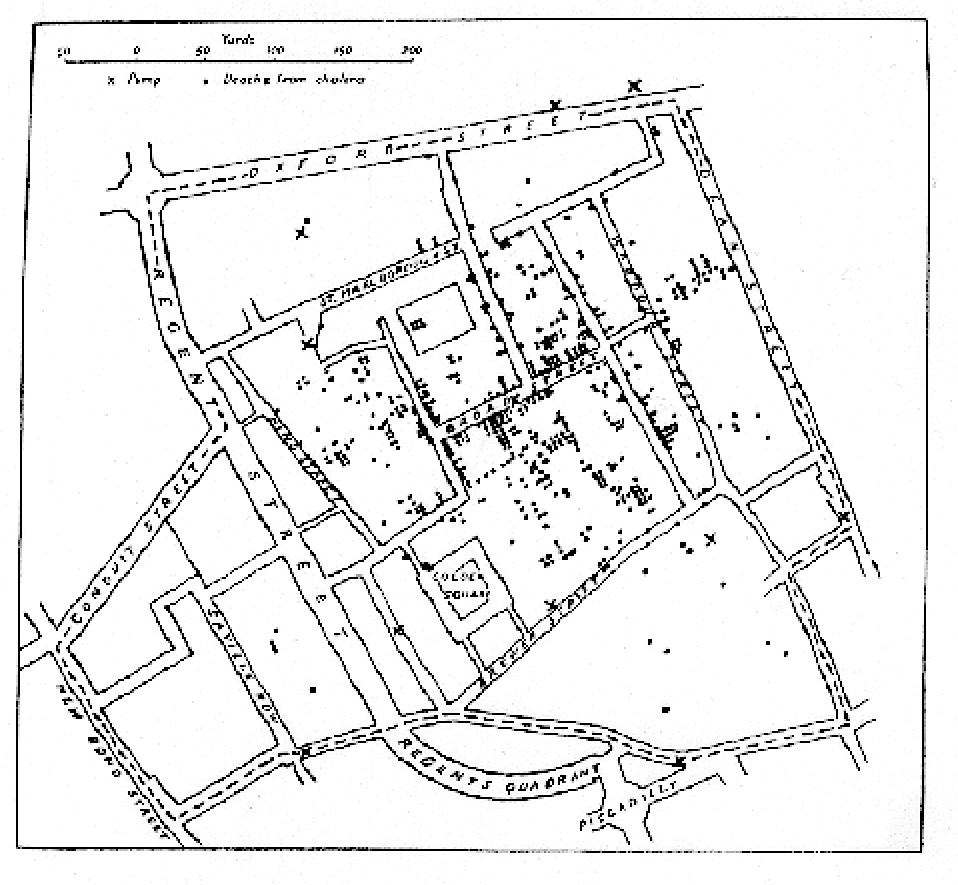
\includegraphics[width=461pt]{sg8_cholera}
\end{center}

\caption[Cholera deaths in central London.]{The distribution of cholera
deaths in central London during September 1854 as plotted by
Dr.~John~Snow. The contaminated water pump which was the source of the
outbreak is located towards the centre of the map, in the middle of
Broad Street. Reproduced from Gilbert\cite{GILBERT}. \label{CHOLERA} }

\end{figure}

% ------------------------

\begin{figure}[htbp]

\begin{center}
\leavevmode
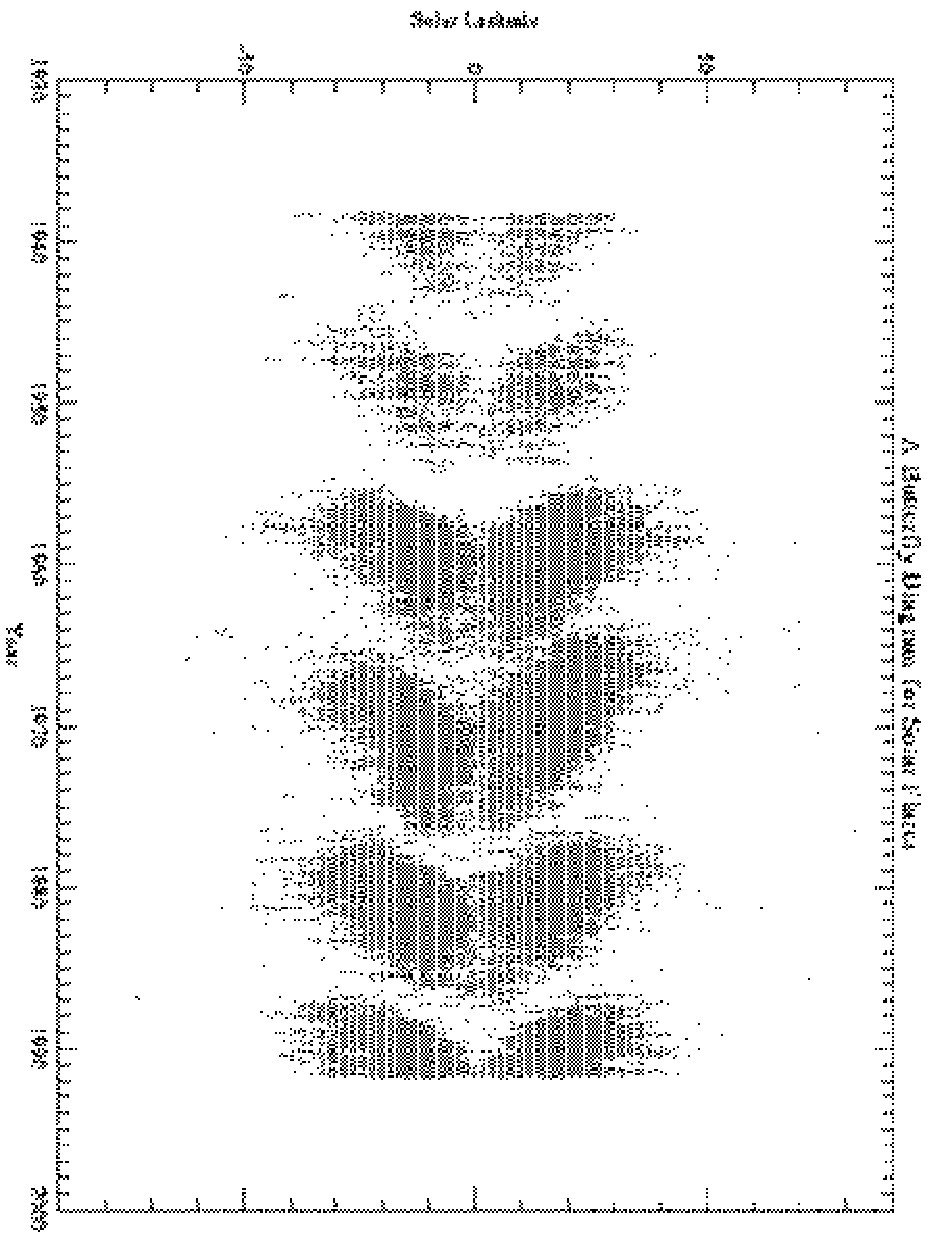
\includegraphics[width=449pt]{sg8_butterfly}
\end{center}

\caption[Butterfly diagram for solar flares.]{Butterfly diagram for
solar flares. Latitude on the solar disk is plotted against time. The
flares show the same characteristic `butterfly' distribution as
sunspots. This plot is due to K.~S.~Balasubramaniam, National Solar
Observatory, Sunspot, New Mexico. \label{SUNSPOT} }

\end{figure}

What has changed in recent years is not the basic idea of using
graphical techniques to represent numerical data, but rather the volume
of such data available. Modern astronomical instrumentation can produce
large and complex datasets comprising megabytes of numbers. Theoretical
models of astronomical phenomena running on powerful modern workstations
or supercomputers can generate similar amounts of data.

Visualisation software is designed to display and explore these enormous
datasets. There are many visualisation packages available, ranging from
large and complex general purpose systems to simpler packages for more
specialised tasks. Some visualisation packages are commercial products,
others are in the public domain. For many years astronomers have used
conventional graphics and image display packages to display and explore
one- and two-dimensional data. Usually visualisation software will offer
only similar facilities for one- and two-dimensional data. However, it
provides much more powerful and sophisticated techniques for the
display of both scalar and vector three-dimensional data.

Visualisation texts often describe one- and two-dimensional graphics
packages as `presentation graphics', assuming that they are principally
used to present finished results (for example, for publication) rather
than to initially explore the data. In astronomy, at least, this
assertion is simply not valid and two-dimensional graphics packages are
used extensively to explore data as well as to present finished results.
Indeed the two-dimensional scatter plot is a standard technique for
exploring data.

The remainder of this document is structured as follows.

\begin{description}

  \item[{\rm Part I}] -- an overview of visualisation techniques to
    help you assess which techniques may be suitable for your data,

  \item[{\rm Part II}] -- a summary of various visualisation packages
   to help you decide which to use.

\end{description}

Starlink recommends the visualisation package IBM Data Explorer (DX) for
general purpose visualisation. It is particularly recommended for the
visualisation of three-dimensional scalar and vector data. It is a
commercial package which costs money. For this reason it is not
automatically available at all Starlink sites, but rather is only
provided at sites which have requested it. DX is briefly described in
Section~\ref{IBMDX} and its use at Starlink sites is documented in
\xref{SUN/203}{sun203}{}\cite{SUN203} and \xref{SC/2}{sc2}{}\cite{SC2}.
Similarly, some sites have bought licences for the Interactive Data
Language (IDL, see Section~\ref{IDL}). Other packages may also be
available. Your site manager should be able to advise on what is
available at your site.

Specialised software for plotting finding charts from astronomical
catalogues is specifically not covered in this document. Starlink
provides the {\tt CHART} package for this purpose and it is described
in SUN/32\cite{CHART}. Another similar program is
\htmladdnormallink{{\bf skymap}}
{http://tdc-www.harvard.edu/software/skymap.html}\cite{SKYMAP}
written by D.~Mink of the Smithsonian Astrophysical Observatory.


\section{Terminology for Types of Data \xlabel{TERMIN} }

Astronomical data can broadly be divided into two different types:
{\bf tabular} and {\bf pixel} data.

{\bf Tabular} datasets are simply tables or lists of values, comprising
measurements for a set of properties (positions, magnitudes, colours
etc.) for a set of objects. The same set of properties are measured for
each object. Astronomical catalogues are simply large tabular datasets.

{\bf Particle} data are an important special case of tabular data where
the properties for each object (or `particle') include two- or
three-dimensional positions. In the context of visualisation software
these positions are usually Cartesian coordinates rather than
spherical-polar celestial coordinates.

{\bf Pixel} datasets comprise a set of measurements on a regularly
spaced grid. The grid may have one, two, three or occasionally more
dimensions. Typically within a programming language a pixel dataset
is represented as an array of the appropriate dimension.

The pixel grid almost invariably represents a set of samples of a
continuous distribution. Often visualisation packages will make a
distinction between the cases where the sampling is a true instantaneous
sample of the underlying distribution at a precisely defined position
and where it represents the average value of the distribution in the
small region defined by the point and its neighbours. However, this
distinction is not important in the context of this document. Similarly
visualisation packages often provide facilities for grids where the points
are not regularly spaced along one or more of the axes (see
Figure~\ref{GRIDS}).

\newpage
\begin{figure}[htbp]
\begin{center}

\begin{picture}(90,50)(0,0)
\thicklines

% Regular grid.

\put(10,10){ \line(1,0){30} }  % Horizontal.
\put(10,15){ \line(1,0){30} }
\put(10,20){ \line(1,0){30} }
\put(10,25){ \line(1,0){30} }
\put(10,30){ \line(1,0){30} }
\put(10,35){ \line(1,0){30} }
\put(10,40){ \line(1,0){30} }

\put(10,10){ \line(0,1){30} }  % Vertical.
\put(15,10){ \line(0,1){30} }
\put(20,10){ \line(0,1){30} }
\put(25,10){ \line(0,1){30} }
\put(30,10){ \line(0,1){30} }
\put(35,10){ \line(0,1){30} }
\put(40,10){ \line(0,1){30} }

\put(10,5){(a) Regular grid}

% Irregular grid.

\put(50,10){ \line(1,0){30} }  % Horizontal.
\put(50,11){ \line(1,0){30} }
\put(50,12){ \line(1,0){30} }
\put(50,14){ \line(1,0){30} }
\put(50,18){ \line(1,0){30} }
\put(50,26){ \line(1,0){30} }
\put(50,40){ \line(1,0){30} }

\put(50,10){ \line(0,1){30} }  % Vertical.
\put(51,10){ \line(0,1){30} }
\put(52,10){ \line(0,1){30} }
\put(54,10){ \line(0,1){30} }
\put(58,10){ \line(0,1){30} }
\put(66,10){ \line(0,1){30} }
\put(80,10){ \line(0,1){30} }

\put(50,5){(b) Irregular grid}

\end{picture}

\caption[Regularly and irregularly spaced grids.]{Regularly and
irregularly spaced grids. \label{GRIDS} }

\end{center}
\end{figure}

Sometimes (but not in this document) the terms `voxel' and `cell' are
used for individual elements of three-dimensional pixel data. A
three-dimensional pixel grid is often referred to as a {\bf data cube}.
This term is somewhat misleading as there is no constraint that the grid
should have the same number of elements in each dimension. Strictly
speaking the term `data cuboid' would be more accurate (that is, the
three-dimensional analogue of a rectangle rather than a square). However,
in this document the more common and familiar term `data cube' will be used.
The term `brick' is also sometimes used as a synonym for a data cube (or
a cuboid subset inside a data cube), though again not in this document.


\cleardoublepage
\markboth{\stardocname}{\stardocname}
\part{Visualisation Techniques}
\markboth{\stardocname}{\stardocname}

\section{Introduction \xlabel{INTRO_TECH} }

This section is a brief general introduction to visualisation techniques,
not tied to any particular software package. It is intended to suggest
techniques that might be appropriate for use on your data. It is largely
based on the review by \htmladdnormallink{Brodlie {\it et al}}
{http://www.agocg.ac.uk:8080/agocg/New/TechReports/VisSyst/dogbook_1.html}\cite{BRODLIE},
the introduction to visualisation by Earnshaw and Wiseman\cite{EARNSHAW},
the report by \htmladdnormallink{Beli\"{e}n {\it et al}}
{http://www.sara.nl/Rik/REPORT.update}\cite{BELIEN} and the notes by
Minty {\it et al}\cite{MINTY}. The report by Beli\"{e}n {\it et
al}\cite{BELIEN} contains a detailed description of a simulation of wave
heating of the solar corona. Many of the features of this visualisation
are typical of visualisations of data generated by theoretical
simulations of astronomical phenomena. I strongly recommend it to anyone
planning to make extensive use of visualisation software to display such
data.

The final product of a visualisation system is a displayed image. Thus
approximations can often be made in the underlying numerical techniques
used to generate the image because the final result does not need to have
high numeric accuracy. This situation differs from generating
theoretical models of astronomical phenomena, where it is usually
important to retain numerical accuracy in intermediate calculations.

First the representation of colour in visualisation systems is briefly
considered, then  the familiar techniques for displaying one- and
two-dimensional data are summarised. The techniques for three-dimensional
scalar and vector data are described in more detail. These techniques are
the characteristic and distinguishing features of contemporary
visualisation packages, and are less likely to be familiar to
astronomers. Visualisation systems usually seem to have the implicit
assumption that in three-dimensional data (particularly pixel data)
the independent variables are Cartesian axes in space. The dependent
variable to be visualised populates this space. It may be either a
scalar quantity such as temperature, pressure or density or a vector
such as velocity or momentum. If the three independent variables are
not Cartesian coordinates  (they might, for example, be spherical or
cylindrical coordinates) then it is usually possible to display them as
though they were Cartesian coordinates, though obviously care must be
taken in interpreting the ensuing visualisations. Finally techniques for
displaying data of higher than three dimensions are considered briefly,
though often such data cannot be visualised adequately. In addition to
their spacial dimensions data to be visualised may also have a temporal
dimension. For example, a sequence of data cubes or particle datasets
might show the evolution of a system over time.

In addition to displaying a single static image another technique which
is often used in visualisation is to show a sequence of images as an
animation or `movie'. The animation may show a series of representations
of the same dataset, such as: the viewpoint being perambulated to
circumnavigate a data cube, a sequence of slices being swept through a
data cube (see Section~\ref{SLICE}) or a sequence of iso-surfaces
(three-dimensional contours; see Section~\ref{ISOSURFACE}) being swept
through a data cube. Alternatively the animation could show genuine
changes in a dynamic system over time, for example, variable or unstable
flow in a fluid. In order to give the impression of smooth motion
the usual rule of thumb is that an animation must be displayed
at a rate of at least twenty-five frames per second. Usually the
individual frames cannot be computed this quickly; they must be
pre-computed, stored and played back as an animation. An animation can
be played back on a conventional computer display such as an X-terminal.
However, even with pre-computed images it is not always possible to
achieve the required display rate. Alternatively, if special equipment
is available, the frames may be stored as analogue images on video tape
and played back using a conventional monitor. This technique ensures
that the animation will play at an adequate rate. Finally, a useful tip
is that often an adequate time step between frames for smooth motion in
an animation is much larger than the necessary time step for accurate
computations of a simulation. Thus, in a complex simulation it is not
necessary to save every time step as a frame for display.

\subsection{Diagrams}

The diagrams reproduced in the paper version of this document do not
adequately reproduce visualisations displayed on a high-quality
graphical output device such as an X-terminal. For example, colour
is not reproduced. On Starlink systems, versions of most of the
diagrams in this section are available as colour GIF files in directory:

\begin{quote}
{\tt /star/examples/sg8}
\end{quote}

and non-Starlink systems in directory:
\begin{quote}
{\tt \$STARLINK\_DIR/examples/sg8}
\end{quote}

The hypertext version of the document includes colour versions of the
diagrams.


\section{Colour Representation \label{COLREP} \xlabel{COLREP} }

The discussion in this section is largely taken from
\htmladdnormallink{Beli\"{e}n {\it et al}}
{http://www.sara.nl/Rik/REPORT.update}\cite{BELIEN}. For a more
comprehensive treatment see, for example, Foley and van Dam\cite{FOLEY1}
and (particularly) Foley {\it et al}\cite{FOLEY2}. The use of colour is
essential in visualisation. Typically a range of values in a dataset are
mapped to a range of colours. However, variations in colour can also be
used to mimic light reflecting off a surface, and thus add depth cues to
an image.

When using visualisation software you will often need to specify colours
or ranges of colours. To do so effectively you need to have some
understanding of the system that the visualisation package uses to
represent colours. There are numerous schemes for representing colours,
both in computer graphics and more generally. Only a few of the ones
commonly used in visualisation software will be discussed here.

The Red-Green-Blue ($RGB$) system is widely used in computer hardware
and you might already be familiar with it. It represents a colour
as three independent components: Red ($R$), Green ($G$) and Blue ($B$).
Typically the components are normalised to the range 0 to 1. $RGB$
colours can be thought of as points in a cube with the three components
as axes. $R=0, G=0, B=0$\, corresponds to black and $R=1, G=1, B=1$\,
corresponds to white. Maximum intensity blue, for example, is $R=0, G=0,
B=1$. Shades of grey lie along the diagonal from the black corner to the
white corner. Other colours occupy intermediate positions in the cube.
Though the $RGB$\, system is conceptually simple, relating $RGB$\,
values to perceived colours is not intuitive.

The Cyan-Magenta-Yellow ($CMG$) system is a variant of the $RGB$\,
system which is widely used in the printing industry. It still
represents a colour as three independent components defining a cube,
but the components are Cyan ($C$), Magenta ($M$) and yellow ($Y$). The
relationship between the $RGB$\, and $CMY$\, systems (for normalised
components) is trivially:

\begin{eqnarray}
C = 1 - R  \nonumber \\
M = 1 - B  \\
Y = 1 - G  \nonumber
\end{eqnarray}

The Hue-Saturation-Value ($HSV$) system was originally introduced by
Smith\cite{SMITH78} and is now widely used in visualisation software,
including Data Explorer. In the $HSV$\, system colours occupy an
inverted cone\footnote{For simplicity the cone is shown with a circular
outline in Figure~\ref{HSV}. Conventionally, for example in Foley and
van~Dam\cite{FOLEY1} and Foley {\it et al}\cite{FOLEY2}, it has an
hexagonal base, with the primary colours and their complements
corresponding to the corners. This difference is not important for the
present discussion.} (see Figure~\ref{HSV}). Within the cone a colour is
a point defined by three components: Hue ($H$), Saturation ($S$) and value
($V$). These three components are defined as follows.

\begin{figure}[htbp]

\begin{center}
\leavevmode
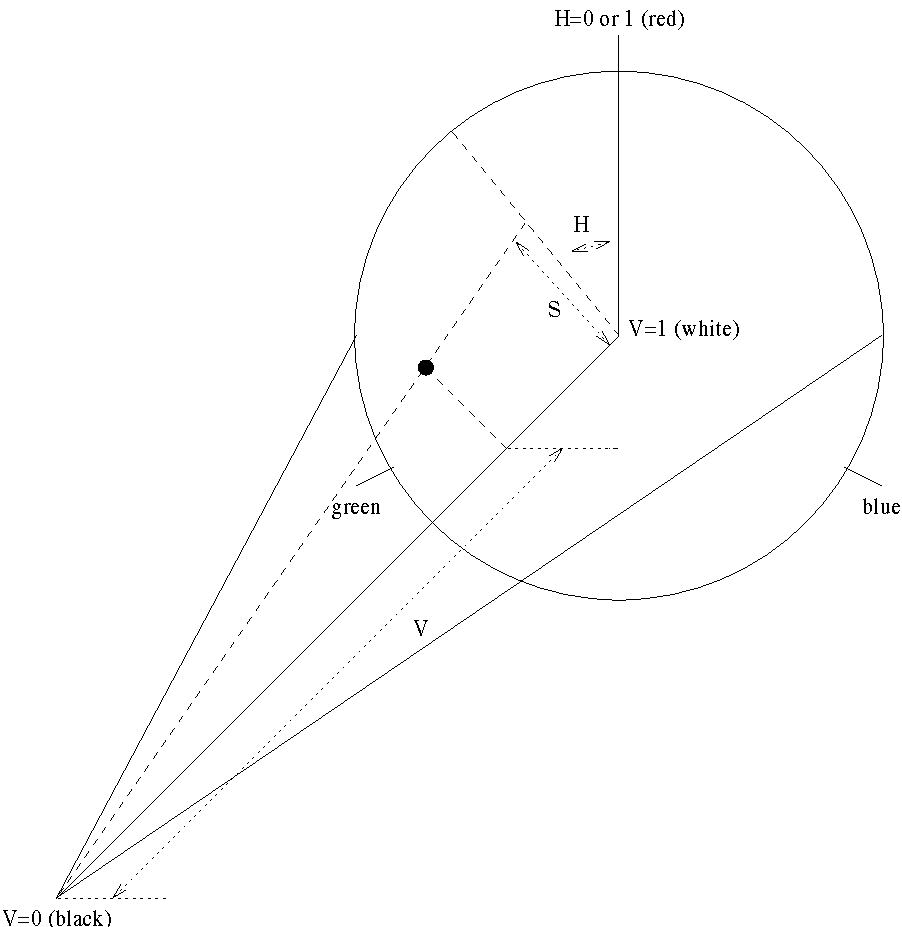
\includegraphics[width=434pt]{sg8_hsv}
\end{center}

\caption[The Hue-Saturation-Value ({\it HSV}) system.]{The
Hue-Saturation-Value ({\it HSV}) system. \label{HSV} }

\end{figure}

\begin{description}

  \item[{\it V}] (or Value) is the distance of the point from the
   apex of the cone, measured along the principal axis. $V=0$\, is the
   apex of the cone and corresponds to black (the values of the other
   components are irrelevant here). A point on the base of the cone has
   $V=1$\, and the point where the principal axis intersects the base
   of the cone corresponds to white. Intermediate points along the
   principal axis correspond to shades of grey.

  \item[{\it H}] (or Hue) is the angle measured around the principal
   axis of the cone. For points on the outer circumference of the
   cone it corresponds to a `pure' colour; $H=0$\, corresponds to red,
   $H=0.333\ldots$\, (or $120^{\circ}$) corresponds to green and
   $H=0.666\ldots$\, (or $240^{\circ}$) corresponds to blue. $H=1$
   completes one rotation and corresponds to red again. Complementary
   colours are on diametrically opposite sides of the cone (that is
   they differ by $180^{\circ}$\, in $H$). Points on the circumference of
   the base of the cone (that is at $V=1$) have a pure colour with maximum
   intensity. Points further up the outside of the cone (that is $V<1)$\,
   have the same `pure' colour as the corresponding colour on the
   circumference of the base, but at a reduced intensity.

  \item[{\it S}] (or Saturation) is the distance from the principal
   axis, projected on to the base of the cone. It measures the purity
   of the colour, that is the extent to which it is diluted with white.
   For a colour lying on the base of the cone $S=0$\, lies on the
   principal axis and corresponds to white and $S=1$\, lies on the edge
   of the cone and corresponds to a pure colour, for example $H=0,
   S=1, V=1$\, is pure red with maximum intensity. Points further up the
   cone (that is $V<1$) have a correspondingly reduced intensity.

\end{description}

The principal advantage of the {\it HSV}\, system is that it
corresponds reasonably closely to human perception of colour and thus
the effects of specifying and manipulating colours in the {\it HSV}\,
system are quite intuitive and predictable. It is possible to transform
between the {\it HSV} and {\it RGB} systems; see Foley and
van~Dam\cite{FOLEY1} and Foley {\it et al}\cite{FOLEY2} for details.
When defining mappings between values in a dataset and colours it is
often useful to remember that the human eye can discriminate hundreds
of different hues but only tens of different values (see for example
MacEachren\cite{MACEACHREN}, p52).


\section{One- and Two-Dimensional Data \xlabel{ONETWOD} }

The techniques for displaying one- and two-dimensional data are well
known. For tabular data they include histograms, scatter plots, line
plots and time series. For pixel data they include pixel image displays
in either grey-scale or false colour, contour maps and carpet plots. The
latter technique might be slightly less familiar; briefly the
intensity of each pixel is represented as a height on the $z$\, axis
and the resulting plane is viewed in perspective from a small distance,
with hidden line removal to improve the appearance (see
Figure~\ref{CARPET}). The name comes from the resemblance to a carpet
draped over an assemblage of bulky objects.

\begin{figure}[htbp]

\begin{center}
\leavevmode
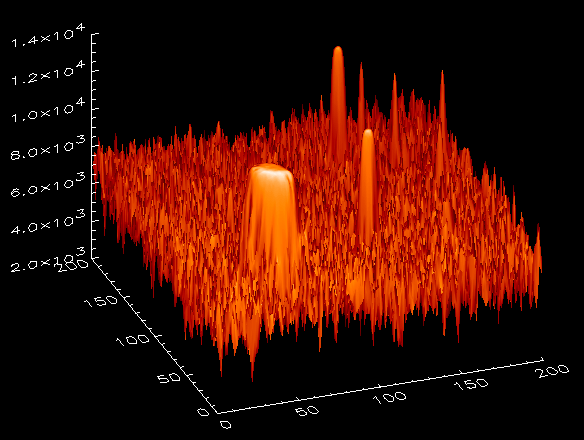
\includegraphics[width=470pt]{sg8_carpet_colour}
\end{center}

\caption[A carpet plot.]{A carpet plot. The plot shows a small region
of a photographic plate taken with the UK Schmidt Telescope at the
Anglo-Australian Observatory, Siding Springs, New South Wales and
digitised with the SuperCOSMOS fast microdensitometer at the Royal
Observatory Edinburgh. The plot was generated with IDL (see
Section~\ref{IDL}). \label{CARPET} }

\end{figure}

Vector data are naturally represented as arrows, with the position of the
base of the arrow corresponding to the position of the datum, the arrow
pointing in the direction of the vector and the length of the arrow
corresponding to the magnitude of the vector. Alternatively (or
additionally) the arrow can be coloured to correspond to the magnitude of
the vector (or any other dependent quantity). These techniques are obviously
applicable to particle data and can also be applied to pixel data. They work
well for small and moderate size datasets, but are less suited for large
datasets where the display can become cluttered because the arrows overlap.
Additional variations on the technique are possible (see Figure~\ref{NSCAT}).


\begin{figure}[htbp]

\begin{center}
\leavevmode
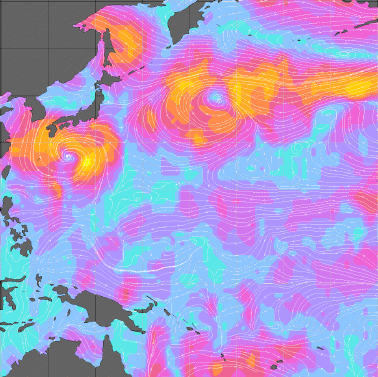
\includegraphics[width=379pt]{sg8_nscat_colour}
\end{center}

\caption[Two-dimensional vector data.]{Two-dimensional vector data.
The image shows wind vectors over the Pacific Ocean south-east of Japan
on the 20th September 1996.  The white arrows show the direction of
the wind and the background colour indicates the speed, with darker
shades of grey corresponding to greater speed.  The data were obtained
with the NASA Scatterometer (NSCAT) on-board the Japanese Advanced Earth
Observing Satellite (ADEOS). \label{NSCAT} }

\end{figure}

Vector pixel data may also be displayed as a series of stream lines.
A stream line is a line everywhere parallel to the direction of the
velocity field. Stream lines and other similar techniques are discussed
further in Section~\ref{VECTOR3D} for three-dimensional vector data.


\section{Three-Dimensional Scalar Data
\label{SCALAR3D} \xlabel{SCALAR3D} }

There are several well developed techniques for displaying data cubes
of three-dimensional pixel data, including slicing, iso-surface
rendering and volume rendering. These techniques are briefly described
below. Finally the less satisfactory techniques for displaying
three-dimensional tabular data are mentioned.

\subsection{Slicing}

In slicing a two-dimensional plane, or `slice', is extracted from the
three-dimensional data cube and displayed as a two-dimensional image.
The slice may be either parallel to one of the axes of the cube or at
an arbitrary orientation. Clearly, while a slice will show detailed
information about the plane being displayed it does not give an
impression of the entire cube.

A simple but surprisingly effective method of visualising the entire
cube is to generate an animation showing a sequence of slices being
swept through the cube parallel to one of the axes. The slice should be
shown in perspective, in its correct position inside the cube, with a
wire grid or set of axes to show the extent of the cube (see
Figure~\ref{SLICE}). The user should be able to control the speed of the
animation, select individual frames for inspection, change the colour
table etc. An animation of this sort is the simplest method of displaying
an entire data cube, but nonetheless can give surprisingly good results.

\begin{figure}[htbp]

\begin{center}
\leavevmode
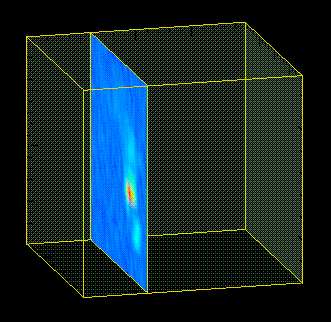
\includegraphics[width=342pt]{sg8_slice_colour}
\end{center}

\caption[Perspective view of a slice in a three-dimensional data
cube.]{Perspective view of a slice in a three-dimensional data cube. The data
cube consists of a stack of radial velocity measurements of the HI 21cm
line over a small region of sky around the North Celestial Pole. The slice
shows the intensity of the emission over the region at a single radial
velocity. The observations were made with the Effelsberg 100m radio
telescope of the Radioastronomisches Institut der Universit\"{a}t Bonn and
are described by Meyerdierks\cite{CLOUDS}. The visualisation was generated
with Data Explorer (see Section~\ref{IBMDX}). \label{SLICE} }

\end{figure}

\subsection{Iso-surface rendering}

In iso-surface rendering (or iso-rendering) a so-called `iso-surface'
corresponding to a given constant value within the data cube is computed
and displayed. An iso-surface is the three-dimensional analogue of a
single contour in a two-dimensional pixel data set. Typically the
iso-surface will be displayed in perspective from a view point some
small distance outside the data cube, and thus usually only one side
of it will be visible (see Figure~\ref{ISOSURFACE}).

\begin{figure}[htbp]

\begin{center}
\leavevmode
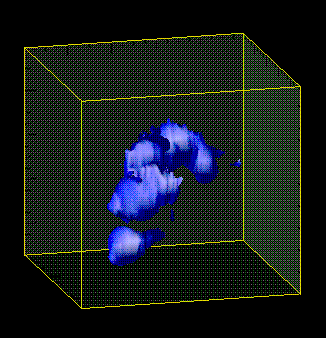
\includegraphics[width=315pt]{sg8_iso_colour}
\end{center}

\caption[Perspective view of an iso-surface in a three-dimensional data
cube.]{Perspective view of an iso-surface in a three-dimensional data
cube. The visualisation shows the same data cube as Figure~\ref{SLICE}.
It was generated with Data Explorer (see Section~\ref{IBMDX}).
\label{ISOSURFACE} }

\end{figure}

A method of visualising the entire data cube is to generate an animation
showing a sequence of iso-surfaces sweeping from the lowest to the
highest data values in the cube (or vice versa). Alternatively, or
additionally, the animation can perambulate the viewing position to
circumnavigate the data cube, thus allowing the user to examine all the
sides of the iso-surface. Again the user should be able to control the
speed of the animation, select individual frames for inspection,
change the colour table etc. Calculating iso-surfaces is a
computationally intensive process and usually it will be necessary to
pre-compute each frame prior to showing the animation, rather than
computing each frame `on-the-fly' as the animation proceeds.

Iso-surface rendering works best where the underlying field varies
smoothly and the iso-surface is relatively simple. In practice in
astronomy this limitation means that it is more suited to displaying
the results of theoretical modelling than observational data. The latter
usually contain a significant amount of noise which tends to break
up the iso-surfaces. This effect is, of course, precisely analogous to
noise tending to break up contours in a two-dimensional contour map.
Also the technique tends to be more successful in cases where the
underlying field is relatively simple, rather than overly complex.

The techniques used to calculate iso-surfaces are beyond the scope of
this document. However, they have been comprehensively reviewed by Ning
and Bloomenthal\cite{NING}.

\subsection{Volume rendering}

Volume rendering is a technique for displaying an entire data cube
without computing any intermediate surfaces. The result is an image
somewhat akin to an X-ray photograph (see Figure~\ref{VREND}).
Various algorithms for volume rendering have been proposed. Two common
ones are ray-casting and `splatting'. Ray casting is summarised below;
see Foley {\it et al}\cite{FOLEY2} for further details. Splatting
is similar to ray casting, though the details are more involved. It
is quicker but produces less accurate results.

\begin{figure}[htbp]

\begin{center}
\leavevmode
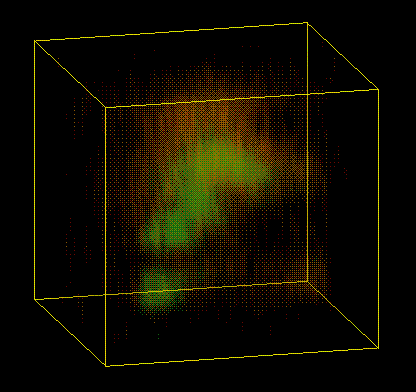
\includegraphics[width=396pt]{sg8_vol_colour}
\end{center}

\caption[Perspective view of a volume rendering of a three-dimensional data
cube.]{Perspective view of a volume rendering of a three-dimensional data
cube. The visualisation shows the same data cube as Figure~\ref{SLICE}.
It was generated with Data Explorer (see Section~\ref{IBMDX}).
\label{VREND} }

\end{figure}

The first step of ray casting (and most volume rendering techniques)
is to generate an `{\it RGBA}\, volume' from the data cube. This
process involves generating a conventional {\it RGB}\, colour (see
Section~\ref{COLREP}) and an opacity, {\it A}, for every pixel in the
data cube. Usually the colour and opacity will be derived from the
value of the pixel using some mapping supplied by the
user\footnote{Usually the user will be required to define the colour
mapping in terms of the {\it HSV}\, system (see Section~\ref{COLREP})
and the visualisation software will automatically transform it to the
{\it RGB}\, system prior to generating the {\it RGBA}\, volume.}. The
opacity is usually normalised to the range 0 to 1, with 0 corresponding
to complete transparency (all light entering the pixel is transmitted
through it) and 1 to a completely opaque pixel (none of the light
entering the pixel is transmitted). Note that pixels can be made invisible
by setting their opacity to 0 and their colour to black.

For every pixel in the output image a ray is projected through the
volume of the data cube. At a set of evenly spaced positions along the
ray the colour and opacity in the data cube are obtained by
interpolating the {\it RGBA}\, array. Starting from an opaque background
behind the data cube and stepping towards the front, the set of colours
and opacities are merged or `composited' to yield the final colour of
the pixel. If $\kappa_{i-1}$\, is the colour of the ray as it enters position
$i$, $c_{i}$ the colour of the position and $a_{i}$\, the opacity
of the position, then the colour of the ray as it leaves the position,
$\kappa_{i}$\, is:

\begin{equation}
\kappa_{i} = \kappa_{i-1} ( 1 - a_{i} ) + c_{i} a_{i}
\end{equation}

Clearly the mappings used to convert pixel values to colours and
opacities will largely determine the appearance of the final image.
In the limit where the mapping is such that all except a narrow range of
pixel values are made invisible (that is, transparent and black) then
the volume rendering will approximate to an iso-surface.

The advantage of volume rendering is that potentially it retains all the
information in the image and no assumptions are made about structure or
surfaces within the data. It is capable of showing faint, complex
filamentary structures in a data cube and is more robust in the presence
of noise than iso-surface rendering. These attributes make it particularly
suitable for visualising astronomical observations, particularly of
tenuous nebul\ae. However, volume rendering is not a simple panacea for
visualising cubes of astronomical data. In order to produce an effective
visualisation it is helpful to have some prior understanding of the
structure of the data and considerable care must be taken in defining
the mapping used to convert pixel values to colours and opacities.
It is usually necessary to experiment in order to produce values suitable
for a given data cube.

A disadvantage of volume rendering is that usually it is very
computationally intensive. Further details of volume rendering
techniques are given by Upson\cite{UPSON}.


\subsection{Particle data}

Particle data can be displayed as points in a perspective plot of the
three-dimensional volume enclosing the dataset. Usually the plot will
include a set of axes or a bounding box. Unfortunately the
three-dimensional position of a point within such a plot is completely
ambiguous (see Figure~\ref{PART3D}).

\begin{figure}[htbp]
\begin{center}

\begin{picture}(60,60)(0,0)
\thicklines

\put(10,10){ \line(1,0){30} } % Front frame.
\put(10,40){ \line(1,0){30} }
\put(10,10){ \line(0,1){30} }
\put(40,10){ \line(0,1){30} }

\put(20,20){ \line(1,0){30} } % Back frame.
\put(20,50){ \line(1,0){30} }
\put(20,20){ \line(0,1){30} }
\put(50,20){ \line(0,1){30} }

\put(10,10){ \line(1,1){10} } % Sides.
\put(10,40){ \line(1,1){10} }
\put(40,10){ \line(1,1){10} }
\put(40,40){ \line(1,1){10} }

\put(11,21){.}
\put(15,18){.}
\put(15,24){.}
\put(15,33,){.}
\put(16,13){.}
\put(17,37){.}
\put(18,28){.}
\put(21,24){.}
\put(23,17){.}
\put(24,43){.}
\put(25,34){.}
\put(25,30){.}
\put(25,24){.}
\put(26,22){.}
\put(27,17){.}
\put(28,33){.}
\put(28,30){.}
\put(27,25){.}
\put(30,37){.}
\put(31,33){.}
\put(29,28){.}
\put(30,24){.}
\put(31,13){.}
\put(33,44){.}
\put(34,38){.}
\put(32,27){.}
\put(34,23){.}
\put(33,17){.}
\put(38,43){.}
\put(38,37){.}
\put(37,32){.}
\put(35,27){.}
\put(38,24){.}
\put(43,32){.}
\put(44,23){.}
\put(36,14){.}
\put(42,16){.}
\put(47,42){.}

\end{picture}

\caption[Perspective view of a schematic three-dimensional particle
data.]{Perspective view of a schematic three-dimensional particle data.
\label{PART3D} }

\end{center}
\end{figure}

There are several techniques which can be used to indicate the position
of the points in three-dimensional space. If there are only a few
points in the data then a set of perpendiculars can be projected from
each datum to one or more of the axes. This technique only works for
small datasets.

For larger datasets the size, brightness or colour of each point can
be used to indicate its distance from the viewing position. In the
first two cases nearer objects are larger or brighter respectively;
the use of colour is more problematic. Alternatively or additionally
an animation can be generated in which the dataset rotates and the
apparent motion of the points gives visual cues about their distance.
None of these techniques is really satisfactory for very large datasets.

\pagebreak
Finally for large datasets it may be possible to bin or
sample\footnote{Binning involves summing the particles inside each of a
grid of cells, where each cell has the same size. In sampling the average
number of particles at a grid of positions is computed. The latter
technique is more robust because the volume used to find the average
can be allowed to vary with the particle density.} the data into a
three-dimensional grid and then display this grid using one of the
methods for pixel data. Whether either of these approaches is practical
or applicable depends on the dataset being investigated.


\section{Three-Dimensional Vector Data
\label{VECTOR3D} \xlabel{VECTOR3D} }

In theory both tabular and pixel three-dimensional vector data can
occur. In practice visualisation systems more often provide facilities
for pixel data. In this case the basic dataset is a data cube of
three-dimensional vectors. These vectors represent an instantaneous
sampling of points in a three-dimensional vector field. Visualising
such a dataset is a complex and difficult task and visualisation
techniques are still evolving in this area. An excellent recent review
is given by Post and van Walsum\cite{POST}. In astronomy
three-dimensional vector data are more likely to result from theoretical
modelling than observations.

Vector fields may be either steady or changing with time. A single data
cube represents a field at an instant of time and is necessarily
equivalent to a steady field. To represent a changing or dynamic field
it is necessary to have a stack of cubes sampling the field at a set of
time steps.

Visualising vectors in a three-dimensional cube is a similar problem
to visualising flows in fluid mechanics. Indeed, many of the
techniques used in vector visualisation are analogues of laboratory
techniques used to study flows in real fluids. Some of the more common
techniques are described briefly below; the discussion is based
on the list of \htmladdnormallink{Brodlie {\it et al}}
{http://www.agocg.ac.uk:8080/agocg/New/TechReports/VisSyst/dogbook_1.html}\cite{BRODLIE}.
The atlas by Van~Dyke\cite{DYKE} contains striking examples of the
laboratory analogues of many of these techniques.

\begin{description}

  \item[Arrows] The most obvious way to represent a data cube of vectors
   is to plot each vector as an arrow. This technique is a simple
   three-dimensional analogue of a two-dimensional arrow plot. The
   direction of the arrow corresponds to the direction of the vector
   and the length of the arrow represents the magnitude of the vector.
   Usually the plot will be shown in three-dimensional perspective,
   viewed from some distance outside the data cube and with axes or a
   bounding box to delimit its extent.

   Unfortunately there are serious problems with this technique. Both
   the position and orientation of an individual arrow within the data
   cube are completely ambiguous (see Figure~\ref{ARROW1}). Also, if
   there is even a moderate number of pixels in the grid the plot can
   become overly crowded, with arrows drawn on top of each other and
   impossible to distinguish (in visualisation jargon this phenomenon
   is known as `occlusion').

  \begin{figure}[htbp]
  \begin{center}

  \begin{picture}(60,60)(0,0)
  \thicklines

  \put(10,10){ \line(1,0){30} } % Front frame.
  \put(10,40){ \line(1,0){30} }
  \put(10,10){ \line(0,1){30} }
  \put(40,10){ \line(0,1){30} }

  \put(20,20){ \line(1,0){30} } % Back frame.
  \put(20,50){ \line(1,0){30} }
  \put(20,20){ \line(0,1){30} }
  \put(50,20){ \line(0,1){30} }

  \put(10,10){ \line(1,1){10} } % Sides.
  \put(10,40){ \line(1,1){10} }
  \put(40,10){ \line(1,1){10} }
  \put(40,40){ \line(1,1){10} }

  \put(26,17){ \vector(1,2){11} } % Arrow.

  \end{picture}

  \caption[Ambiguous arrow in a data cube.]{Ambiguous arrow in a data cube.
  \label{ARROW1} }

  \end{center}
  \end{figure}

   The crowding can be reduced by averaging neighbouring vectors and
   just displaying the result. Another method of both reducing the crowding
   and indicating the positions of the vectors is to just show vectors
   on a single slice or surface in the data cube. A better indication of
   the direction of the vectors can be given either by drawing, for each
   vector, additional arrows for its three components or by drawing the
   arrow as a three-dimensional object (see Figure~\ref{ARROW2}).
   Rather bizarrely such three-dimensional arrows are sometimes referred
   to as `rockets'. Both these techniques worsen the problem of
   overcrowding within the plot. In summary, arrow plots are not usually
   very satisfactory, even for moderately sized datasets.

  \begin{figure}[htbp]

  \begin{center}
  \leavevmode
  
\includegraphics[width=129pt]{sg8_arrow}
  \end{center}

  \caption[An arrow drawn as a three-dimensional object.]{An arrow drawn
   as a three-dimensional object.
  \label{ARROW2} }

  \end{figure}

  \item[Path lines or particle advection] This technique is the analogue
   of the laboratory technique in which a light emitting particle is
   introduced into the flowing fluid and its progress filmed over a
   specified time interval. Using illuminated particles to trace fluid
   flows is, of course, a familiar technique in astronomy (see
   Figure~\ref{HALLEY}).

  \begin{figure}[htbp]

  \begin{center}
  \leavevmode
  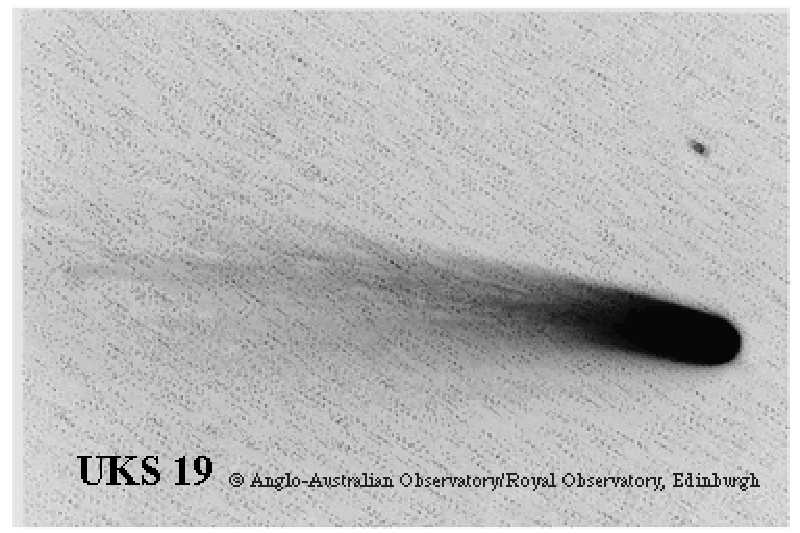
\includegraphics[width=385pt]{sg8_halley_grey}
  \end{center}

  \caption[Comet Halley.]{Comet Halley photographed on 12th March 1986
   by the UK Schmidt Telescope. \label{HALLEY} }

  \end{figure}

  \item[Stream lines] This technique displays the flow as lines
   everywhere parallel to the velocity field. The relative spacing
   of the lines indicates the speed of the flow. For steady flows
   path lines and stream lines are identical.

  \item[Stream ribbons] Stream ribbons are a variation of stream lines
   in which two adjacent stream lines are displayed as a ribbon. This
   approach shows twists in the velocity field which are not visible
   from simple stream lines.

  \item[Stream surfaces] Stream surfaces are a further variation of
   stream lines in which several lines are joined to form a surface.

  \item[Time lines] This technique is the analogue of a laboratory
   technique in which small particles (often hydrogen bubbles) are
   released into the fluid and their subsequent positions monitored.
   Often a line of bubbles will be introduced perpendicular to the
   flow and the line will be displayed as it subsequently distorts,
   advanced by the flow.

  \item[Streak lines] In laboratory work a streak line is a line of
   dye injected into the flow from a fixed point for a given duration.
   The resulting line of dye in the fluid traces the flow. In a
   steady flow the line traces a stream line.

   In computational visualisation the term is used rather loosely;
   sometimes to refer to a line of particles whose positions are traced
   as they follow the flow, sometimes to indicate particle paths in a
   time varying flow.

  \item[Topology methods] In this technique critical points in the
   velocity field where the vector is zero are identified and
   classified as sources, sinks, etc. The critical points are connected
   to divide the flow into regions with similar properties. This
   technique is described by Helman and Hesselink\cite{HELMAN}. It is
   not widely available in visualisation systems, but is included in
   the FAST visualisation environment developed at the NASA Ames
   Research Center (see Section~\ref{FAST}).

  \item[Scalar quantities] It is possible to compute scalar quantities
   for the vector field such as the magnitude of the velocity or the
   magnitude of the vorticity (defined as $\nabla  \times velocity$)
   and display them using the techniques for three-dimensional scalar
   data cubes (see Section~\ref{SCALAR3D}). How useful this approach
   will be depends on the problem being tackled.

\end{description}


\section{Higher Dimensions and Additional Dependent Quantities
\xlabel{HIGHER} }

In general it is not possible to satisfactorily display datasets of
higher than three dimensions in a single image. It is possible to extract
one-, two- or three-dimensional subsets from the data and display them in
the normal fashion. Animations give a usable representation of a fourth
dimension.

A carpet plot (in two dimensions) or iso-surface (in three dimensions)
can be coloured to represent the variation of a second dependent
quantity. For example an iso-surface might be computed along a constant
gas pressure within a data cube and it could be coloured to show the
temperature variation across the iso-surface. Alternatively (or
additionally) another dependent variable can be shown by positioning
`glyphs' such as circles or spheres over the iso-surface. Their size
or colour varies with the dependent variable. Obviously too many such
glyphs cannot be included or the plot will become crowded. Similarly in a
particle plot the colour, size and plotting symbol can be used to indicate
the variation of an additional quantity (assuming that they are not being
used to show distance).


\pagebreak
\markboth{\stardocname}{\stardocname}
\part{Visualisation Packages}
\markboth{\stardocname}{\stardocname}

\section{Choosing a Package \xlabel{CHOOSE} }

This section is intended to help you to choose a visualisation package
which is suitable for your data. There are many visualisation packages
available. In 1992 Earnshaw and Wiseman\cite{EARNSHAW} were able to
list twelve commercial and eight public domain major packages and there
are many more specialised ones. This document will consider only a few
systems, concentrating on either commercial packages which are likely to
be available on Starlink systems or public domain packages which you
should be able to obtain and install. This approach does not, of course,
mean that other systems are not useful. On the contrary, you may well
find a system which though not mentioned here is extremely useful for
your purposes. Subsequent sections give brief details of individual
packages, including a summary of the package and, where appropriate,
details of how to obtain it and information about it.
\begin{latexonly}
A longer list of visualisation systems and related information can
be accessed on-line via the Web at URL:
\begin{quote}
{\tt http://www.roe.ac.uk/acdwww/vissys/index.html}
\end{quote}
\end{latexonly}
\begin{htmlonly}
A longer list of
\htmladdnormallink{visualisation systems and related information}
{http://www.roe.ac.uk/acdwww/vissys/index.html} is also available.
\end{htmlonly}
Also there may be useful information in the usenet news group {\tt
comp.graphics.visualization} which is intended for general discussion
about visualisation.

The more powerful visualisation systems are complicated and involved
tools. It is necessary to invest a certain amount of time to learn how
to use them effectively. Typically generating an animation is a
non-trivial operation involving writing a `program' to import the data,
transform them and generate the visualisation. The programming involved
may well be disguised as positioning boxes within a window using the
cursor and joining them with multi-coloured lines, but nonetheless it is
still, in essence, programming.

The various visualisation systems described in the following sections
fall into the following broad categories:

\begin{description}

  \item[visual programming] (in which icons representing specific
   functions are positioned on a canvas to construct a `network' or
   `program' to generate some specific visualisation): DX, AVS,
   Khoros,

  \item[scripting or command languages:] IDL, PV-WAVE,

  \item[specialised applications:] XGobi, tipsy.

\end{description}

To find a package suitable for your needs you should use the decision
tree in Figure~\ref{DECPART} for particle data and in
Figure~\ref{DECPIX} for pixel data.
\begin{latexonly}
Table~\ref{STARDOC} lists the Starlink documentation for the packages
mentioned in these figures.
\end{latexonly}

\begin{figure}[htbp]

\begin{verbatim}
If the data are one- or two-dimensional then
   XGobi, IDL, PV-WAVE, PONGO, SM, etc.
   PGPLOT (subroutine library)
else if the data are three-dimensional
   If speed of display is important then
      TIPSY
   else
      XGobi, IBM DX
   end if
else the data are higher than three-dimensional
   XGobi and display just three columns
end if
\end{verbatim}

\caption[Decision tree to find a package for visualising particle
data.]{Decision tree to find a package for visualising particle data.
\label{DECPART} }

\end{figure}

% ---------------------

\begin{figure}[htbp]


\begin{verbatim}
If the data are scalar then
   If the data are one- or two-dimensional then
      KAPPA, Figaro, SAOIMAGE, IDL, PV-WAVE etc.
   else if the data are three-dimensional
      IBM DX, (IDL, PV-WAVE, Khoros)
   else the data are higher than three-dimensional
      Use NDFCOPY or COMPAVE in KAPPA to extract a one-, two- or
      three-dimensional subset and proceed as for one-, two- or
      three-dimensional data.
   end if
else the data are vector
   If you want to use the topology method then
      FAST (from NASA Ames).
   else
      If the data are one- or two-dimensional then
         IBM DX, (IDL, PV-WAVE, Khoros)
      else if the data three-dimensional
         IBM DX
      else the data are higher than three-dimensional
         Nothing suitable.
      end if
   end if
end if
\end{verbatim}

\caption[Decision tree to find a package for visualising pixel
data.]{Decision tree to find a package for visualising pixel data.
\label{DECPIX} }

\end{figure}


% ---------------------

\begin{latexonly}
\begin{table}[htbp]

\begin{center}
\begin{tabular}{llc}
Package      & Starlink Document &  Reference \\ \hline
Figaro       & SUN/86   & \cite{FIGARO}   \\
KAPPA        & SUN/95   & \cite{KAPPA}    \\
PGPLOT       & SUN/15   & \cite{PGPLOT}   \\
PONGO        & SUN/137  & \cite{PONGO}    \\
SAOIMAGE     & SUN/166  & \cite{SAOIMAGE} \\
SM           & MUD/160  & \cite{MUD160}   \\
             & MUD/159  & \cite{MUD159}   \\
\end{tabular}
\end{center}

\caption[Starlink documentation for packages mentioned in the decision
trees.]{Starlink documentation for packages mentioned in the decision
trees. \label{STARDOC} }

\end{table}
\end{latexonly}

\begin{htmlonly}

The Starlink documentation for the packages mentioned in these figures
is as follows:


\begin{itemize}

  \item \xref{Figaro}{sun86}{}:    SUN/86\cite{FIGARO},
  \item \xref{KAPPA}{sun95}{}:     SUN/95\cite{KAPPA},
  \item \xref{PGPLOT}{sun15}{}:    SUN/15\cite{PGPLOT},
  \item \xref{PONGO}{sun137}{}:    SUN/137\cite{PONGO},
  \item \xref{SAOIMAGE}{sun166}{}: SUN/166\cite{SAOIMAGE},
  \item SM: MUD/160\cite{MUD160},  MUD/159\cite{MUD159}.

\end{itemize}

\end{htmlonly}

The following general points should be borne in mind.

\begin{enumerate}

  \item There are numerous packages for displaying one- and
   two-dimensional data in addition to the ones shown, including:
   Asterix, QDP, UNIRAS, MIDAS, IRAF, {\it et seq. ad nauseam}.

  \item Starlink recommends IBM Data Explorer (see Section~\ref{IBMDX})
   for general purpose visualisation and particularly for
   three-dimensional scalar and vector data. However, it is a
   commercial product and it will not necessarily be available at your
   site. Your site manager should be able to advise.

  \item IDL (see Section~\ref{IDL}) is quite widely used in astronomy
   and it may well be available at your site. Again your site manager
   should be able to advise. It has quite good facilities for displaying
   three-dimensional scalar data, but is not recommended for
   three-dimensional vector data.

  \item PV-WAVE (see Section~\ref{PVWAVE}) is quite similar to IDL, but
   perhaps has more powerful applications. However, it is not widely
   used in astronomy and there is unlikely to be a copy at your site.
   The reasons why PV-WAVE is less used than IDL in astronomy are
   probably partly historical (IDL has been around for longer) and
   partly because PV-WAVE seems, on balance, more expensive.

  \item Though, strictly speaking, Khoros (see Section~\ref{KHOROS}) is
   not available in the public domain, it is usually available free of
   charge (though there is a charge for paper copies of the manuals).
   Nonetheless Khoros is a complex and sophisticated package, and like
   similar commercial packages it is necessary to invest a certain
   amount of time to learn to use it effectively. Also it is
   unreasonable to expect the same level of support for Khoros as for
   a commercial product.

\end{enumerate}


\section{IBM Data Explorer \label{IBMDX} \xlabel{IBMDX} }

IBM Data Explorer (DX) is a general-purpose software package for data
visualisation and analysis. It employs a data-flow driven client-server
execution model and provides a comprehensive range of data manipulation,
visualisation and display functions. Visualisations can be generated
using a visual programming editor or a text-based scripting language.
DX is the visualisation package recommended by Starlink, particularly
for three-dimensional scalar and vector data. Starlink has produced a
set of enhancements to DX. If you are using DX at a Starlink site then
these enhancements should be available automatically. The use of DX at
Starlink sites and the Starlink enhancements to DX are documented in
\xref{SUN/203}{sun203}{}\cite{SUN203}.

DX is produced by IBM. It can be obtained from IBM or any IBM dealer.
An educational discount is usually available. Because it is the
visualisation package recommended by Starlink there are special
arrangements for obtaining a copy at Starlink sites. Appendix~A of
\xref{SUN/203}{sun203}{}\cite{SUN203} gives the details.

\begin{latexonly}
Further details can be obtained via the Web at URL:

\begin{quote}
{\tt http://www.roe.ac.uk/acdwww/vissys/dx.html}
\end{quote}
\end{latexonly}

\begin{htmlonly}
\htmladdnormallink{Further details}
{http://www.roe.ac.uk/acdwww/vissys/dx.html}.
\end{htmlonly}


\section{AVS \label{AVS} \xlabel{AVS} }

Application Visualization System (AVS) is a general-purpose software
package for data visualisation and analysis. It provides a comprehensive
range of visualisation functions. It includes a visual computing
environment for application development and a set of `ready to use'
applications for common visualisations. AVS is a well established
product with a substantial customer base, although it is currently
undergoing major enhancements in order to incorporate various recent
developments in scientific visualisation. It is not widely used in
astronomy.

AVS is produced by Advanced Visual Systems Inc.\ of 300 Fifth Ave.
Waltham, Massachusetts 02154, United States of America. Advanced Visual
Systems has a subsidiary in the United Kingdom. Its address is:
AVS/UNIRAS Ltd, Montrose House, Chertsey Boulevard, Hanworth Lane,
Chertsey, Surrey, KT16 9JX.

\begin{latexonly}
Further details can be obtained via the Web at URL:

\begin{quote}
{\tt http://www.roe.ac.uk/acdwww/vissys/avs.html}
\end{quote}
\end{latexonly}

\begin{htmlonly}
\htmladdnormallink{Further details}
{http://www.roe.ac.uk/acdwww/vissys/avs.html}.
\end{htmlonly}


\section{Khoros \label{KHOROS} \xlabel{KHOROS} }

Khoros is a powerful, integrated software environment for performing
image and signal processing, data exploration and visualisation. It
includes a visual programming language, a suite of software development
tools that extend the visual language, an interactive user interface
editor, an interactive image display package, two- and three-dimensional
 plotting, and an extensive suite of image processing, data manipulation,
visualization, geometry and matrix operators. It is described by
Rasure and Kubica\cite{RASURE}.

Khoros is protected by copyright and is strictly speaking not available
in the public domain. However, it is usually available free of charge.
Khoros is a complex and sophisticated package, and like similar
commercial packages it is necessary to invest a certain amount of time
to learn to use it effectively.

Khoros is developed by Khoral Research, Inc.\ (KRI) of 6001 Indian
School Road NE, Suite 200, Albuquerque, New Mexico 87110-4139, United
States of America. Copies of Khoros can be obtained from various anonymous
ftp sites.

\begin{latexonly}
Further details can be obtained via the Web at URL:

\begin{quote}
{\tt http://www.roe.ac.uk/acdwww/vissys/khoros.html}
\end{quote}
\end{latexonly}

\begin{htmlonly}
\htmladdnormallink{Further details}
{http://www.roe.ac.uk/acdwww/vissys/khoros.html}.
\end{htmlonly}


\section{IDL \label{IDL} \xlabel{IDL} }

Interactive Data Language (IDL) is not simply a visualisation package
{\it per se}, but rather is intended for interactive data analysis as
well as for the visualisation of scientific and engineering data.
Consequently it is very flexible and powerful and its usefulness is not
limited to visualisation.

The basis of IDL is a combined command and programming language similar
to Fortran, but more powerful and easier to use. It contains many
intrinsic functions for image and data processing and display (though
unfortunately its facilities for visualising three-dimensional vector
data are limited). Doing anything non-trivial using IDL is definitely
`programming', though it is a simple and straightforward language to
program in. Indeed it achieves the impressive double feat of
simultaneously being much more powerful and easy-to-use than Fortran
while having a minimal learning curve for someone already familiar with
Fortran.

IDL has achieved a significant though not very high level of use in
astronomy, though it is used extensively in solar physics and gamma-ray
astronomy. A number of Starlink sites have bought IDL licences, so it
may be available at your site.  Appendix B of
\xref{SUN/55}{sun55}{}\cite{SUN55} describes how to import data in the
Starlink NDF format into IDL.

IDL is produced by Research Systems Inc, 2995 Wilderness Place, Suite
203, Boulder, Colorado 80301, United States of America.  In the United
Kingdom it is sold by Floating Point Systems UK Ltd, Ash Court, 23, Rose
Street, Wokingham, Berkshire, RG11 1XS. For academic users in the
United Kingdom an educational discount is available under a CHEST
agreement.

\begin{latexonly}
Further details can be obtained via the Web at URL:

\begin{quote}
{\tt http://www.roe.ac.uk/acdwww/vissys/idl.html}
\end{quote}
\end{latexonly}

\begin{htmlonly}
\htmladdnormallink{Further details}
{http://www.roe.ac.uk/acdwww/vissys/idl.html}.
\end{htmlonly}


\section{PV-WAVE \label{PVWAVE} \xlabel{PVWAVE} }

PV-WAVE is a data analysis and visualisation package for scientific
and engineering data very similar to IDL (see Section~\ref{IDL}).
Indeed PV-WAVE and IDL share the same basic language and have a common
ancestry. PV-WAVE seems to be a more developed product, with more
advanced applications than IDL, for example the {\it Point \& Click}\,
GUI-based applications for data exploration and image and signal
processing.

The following extract from the IDL and PV-WAVE FAQ explains the
relationship between the two packages.

\begin{quote}
`Around the time that the Unix version of IDL first became
available (1988), Precision Visuals Inc.\ (PVI) entered into an agreement
with RSI [the vendors of IDL] under which they enhanced and resold IDL
under the name PV~WAVE. In September of 1990, they exercised an option in
that agreement that resulted in the following:

\begin{itemize}

  \item They received a copy of the IDL source code as it existed in
   September 1990 in return for a one-time payment to RSI.

  \item The connection between RSI and PVI was severed.

\end{itemize}

IDL and PV~WAVE are now on separate development tracks. Each company
enhances, supports, and maintains its own product.

PVI has since merged with IMSL and is now Visual Numerics, Inc.\ (VNI).'
\end{quote}

PV-WAVE is produced by Visual Numerics Inc, 6230 Lookout Road, Boulder,
Colorado 80301, United States of America.  Visual Numerics Inc.\ have an
office in the United Kingdom. Its address is: New Tithe Court, 23,
Datchet Road, Slough, Berkshire, SL3 7LL. For academic users in the
United Kingdom an educational discount is available under a CHEST
agreement.

PV-WAVE seems to be little used in astronomy.
\begin{latexonly}
Further details can be obtained via the Web at URL:

\begin{quote}
{\tt http://www.roe.ac.uk/acdwww/vissys/pvwave.html}
\end{quote}
\end{latexonly}

\begin{htmlonly}

\htmladdnormallink{Further details}
{http://www.roe.ac.uk/acdwww/vissys/pvwave.html}.
\end{htmlonly}


\section{XGobi \label{XGOBI} \xlabel{XGOBI} }

XGobi is an extremely easy-to-use public domain package for plotting
scatterplots of multi-dimensional tabular data. It is produced by
Bellcore Inc.\ of New Jersey. It can plot two- and three-dimensional
scatterplots and the three-dimensional plots can be rotated in real time.
All the plots can be zoomed, panned etc. Data are read from ASCII text
files which makes importing data very easy.

\begin{latexonly}
Further details can be obtained via the Web at URL:

\begin{quote}
{\tt http://www.roe.ac.uk/acdwww/vissys/xgobi.html}
\end{quote}
\end{latexonly}

\begin{htmlonly}
\htmladdnormallink{Further details}
{http://www.roe.ac.uk/acdwww/vissys/xgobi.html}.
\end{htmlonly}


\section{TIPSY \label{TIPSY} \xlabel{TIPSY} }

TIPSY is a public domain package written at the University of
Washington for displaying three-dimensional scatterplots of particle
data. Its principal advantage is the speed of display when such a
plot is being rotated in real time. You would probably only choose to
use it if this display speed was important to you. TIPSY was designed
for displaying the results of $n$-body cosmological simulations and it
contains some specialised functionality for use with such data.

\begin{latexonly}
Further details can be obtained via the Web at URL:

\begin{quote}
{\tt http://www.roe.ac.uk/acdwww/vissys/tipsy.html}
\end{quote}
\end{latexonly}

\begin{htmlonly}
\htmladdnormallink{Further details}
{http://www.roe.ac.uk/acdwww/vissys/tipsy.html}.
\end{htmlonly}


\section{FAST \label{FAST} \xlabel{FAST} }

Flow Analysis Software Toolkit (FAST) is a software environment for
analysing three-dimensional data. It contains the usual facilities for
visualising such data (for example, slices, iso-surfaces and particle
traces) but it is unusual that it also has an implementation of the
critical points technique for analysing a vector field (see
Section~\ref{VECTOR3D}). It has a highly interactive interface and
comprises a set of applications with minimal overlapping functionality
but sharing a common data structure. FAST seems to be more concerned
with simulating air flows around aircraft than modelling natural
phenomena.

FAST is developed by the Numerical Aerodynamics Simulation (NAS)
Division at the NASA Ames Research Center, Moffett Field, California
94035-1000, United States of America. FAST is sold commercially, but is
offered to academic users at a much reduced price. Previously it was
available only to users in the United States, though now it is available
worldwide.

\begin{latexonly}
Further details can be obtained via the Web at URL:

\begin{quote}
{\tt http://www.roe.ac.uk/acdwww/vissys/fast.html}
\end{quote}
\end{latexonly}

\begin{htmlonly}
\htmladdnormallink{Further details}
{http://www.roe.ac.uk/acdwww/vissys/fast.html}.
\end{htmlonly}


% \pagebreak
% \part{Importing Data}

% (to be added)

\newpage
\section{Acknowledgments \xlabel{ACK} }

The following people have kindly supplied either complete diagrams
or data which were used to generate visualisations: Figures~\ref{SLICE},
\ref{ISOSURFACE} and \ref{VREND}, H.~Meyerdierks (Institute for
Astronomy, University of Edinburgh); Figure~\ref{CHOLERA},
E.~Minty (Edinburgh Parallel Computer Centre); Figure~\ref{SUNSPOT},
K.~S.~Balasubramaniam (National Solar Observatory, Sunspot, New Mexico);
Figure~\ref{CARPET}, H.T.~MacGillivray (Royal Observatory Edinburgh).
Figure~\ref{HALLEY} is courtesy of the Anglo-Australian Observatory and
the Royal Observatory Edinburgh.

M.D.~Lawden (Starlink) made several useful comments on a draft version of
the document.

% \section{References}

\addcontentsline{toc}{section}{References}
\begin{thebibliography}{99}

  \bibitem{CHART} P.M.~Allan, 1989, SUN/32.12, {\it CHART --- Finding
   Chart and Stellar Data System} (Starlink).

  \bibitem{BELIEN} S.~Beli\"{e}n, S.~Poedts, H.~Goedbloed, H.~Spoelder,
   A.~Emmen, J.~Hollenberg and R.~Leenders, (revised) 1996,
   {\it Comparison of Visualisation Techniques and Packages with
   Applications to Plasma Physics}, available via the Web from URL:
   {\tt http://www.sara.nl/Rik/REPORT.update}

  \bibitem{SUN203} D.S.~Berry, G.J.~Privett and A.C.~Davenhall, 1997,
   SUN/203.2, {\it DX --- IBM Data Explorer for Data Visualisation}\,
   (Starlink).

  \bibitem{BRODLIE} K.W.~Brodlie, J.R.~Gallop, A.J.~Grant, J.~Haswell,
   W.T.~Hewitt, S.~Larkin, C.C.~Lilley, H.~Morphet, A.~Townend,
   J.~Wood and H.~Wright, 1995, {\it Review of Visualization Systems},
   Advisory Group on Computer Graphics Technical Report (Loughborough
   University of Technology: Loughborough, Leicestershire). Also
   available via the Web from URL: {\tt
   http://www.agocg.ac.uk:8080/agocg/New/TechReports/VisSyst/dogbook\_1.html}

  \bibitem{KAPPA} M.J.~Currie, 1995, SUN/95.9, {\it KAPPA --- Kernel
   Application Package}\, (Starlink).

  \bibitem{SUN55} M.J.~Currie, G.J.~Privett and A.J.~Chipperfield,
   1995, SUN/55.6, {\it CONVERT A Format-conversion Package}\, (Starlink).

  \bibitem{SC2} A.C.~Davenhall, 1997, SC/2.2, {\it The DX Cookbook}\,
   (Starlink).

  \bibitem{DYKE} M.~Van~Dyke, 1982, {\it An Album of Fluid Motion}\,
   (The Parabolic Press: Stanford, California).

  \bibitem{EARNSHAW} R.A.~Earnshaw and N.~Wiseman, 1992, {\it An
   Introductory Guide to Scientific Visualization}\,
   (Springer-Verlag: Berlin).

  \bibitem{FOLEY1} J.D.~Foley and A.~van~Dam, 1982, {\it Fundamentals
   of Interactive Computer Graphics}\, (Addison-Wesley: Reading,
   Massachusetts).

  \bibitem{FOLEY2} J.D.~Foley, A.~van~Dam, S.K.~Feiner and J.F.~Hughes,
   1992, {\it Computer Graphics, Principles and Practice}\,
   (Addison-Wesley: Reading, Massachusetts).

  \bibitem{GILBERT} E.W.~Gilbert, 1958, `Pioneer Maps of Health and
   Disease in England', {\it Geographical Journal}, {\bf 124},
   pp172--183.

  \bibitem{HAMMING} R.W.~Hamming, 1962, {\it Numerical Methods for
   Scientists and Engineers}\, (McGraw-Hill: New York).

  \bibitem{PONGO} P.~Harrison, P.~Rees and P.~Draper, 1996, SUN/137.5,
   {\it PONGO --- A Set of Applications for Interactive Data Plotting}\,
   (Starlink).

  \bibitem{HELMAN} J.L.~Helman and L.~Hesselink, 1989,
   `Representation and Display of Vector Field Topology in Fluid Flow
   Data Sets', {\it IEEE Computer}, {\bf 22}, No. 8, pp27-36.

  \bibitem{MUD160} R.~Lupton and P.~Monger, 1995, MUD/160.1, {\it
   The SM Tutorial}\, (Princeton and McMaster Universities; reprinted
   by Starlink).

  \bibitem{MUD159} R.~Lupton and P.~Monger, 1995, MUD/159.1, {\it
   SM --- Interactive Plotting Program, 2.3.1}\, (Princeton and McMaster
   Universities; reprinted by Starlink).

  \bibitem{MACEACHREN} A.M.~MacEachren, 1995, {\it How Maps Work}\,
   (The Guilford Press: New York).

  \bibitem{CLOUDS} H.~Meyerdierks, 1992, {\it Astron. \& Astrophys},
   {\bf 253}, pp515--520.

  \bibitem{SKYMAP} D.~Mink. Details of {\bf skymap} can be obtained
   via the Web from URL:
   {\tt http://tdc-www.harvard.edu/software/skymap.html}

  \bibitem{MINTY} E.~Minty, P.~Maccallum, J.~Fisher and
   A.~Hondroudakis, 1995, {\it Scientific Visualisation: A Practical
   Introduction}, version 2.0 (Edinburgh Parallel Computing Centre
   course notes: Edinburgh).

  \bibitem{SAOIMAGE} R.~Morris and G.J.~Privett, 1995, SUN/166.3,
   {\it SAOIMAGE --- Astronomical Image Display} (Starlink).

  \bibitem{NING} P. Ning and J. Bloomenthal, 1993, `An Evaluation of
   Implicit Surface Tilers', {\it IEEE Computer Graphics and
   Applications}, {\bf 13}, No. 6, pp33--41.

  \bibitem{POST} F.H.~Post and T.~van~Walsum, 1993, {\it Fluid Flow
   Visualization}, in {\it Focus on Scientific Visualization}, eds.
   H.~Hagen, H.~M\"{u}ller and G.M.~Nielson (Springer-Verlag: Berlin),
   pp1--40.

  \bibitem{RASURE} J.~Rasure and S.~Kubica, 1994, {\it The Khoros Application
   Development Environment} in {\it Experimental Environments for
   Computer Vision and Image Processing}, eds H.I.~Christensen and
   J.L.~Crowley (World Scientific: Singapore)  pp1--32.

  \bibitem{ROBIN} H.~Robin, 1992, {\it The Scientific Image From Cave
   to Computer}\, (Harry~N.~Abrams Inc: New York).

  \bibitem{FIGARO} K.~Shortridge, H.~Meyerdierks, M.J.~Currie and
   M.J.~Clayton, 1996, SUN/86.12, {\it FIGARO --- A General Data
   Reduction System} (Starlink).

  \bibitem{SMITH78} A.R.~Smith, 1978, `Color Gamut Transform Pairs',
   SIGGRAPH '78 Proceedings, published as {\it Computer Graphics},
   {\bf 12}(3), pp12-19.

  \bibitem{PGPLOT} D.L.~Terrett, 1995, SUN/15.6 {\it PGPLOT ---
   Graphics Subroutine Library}\, (Starlink).

  \bibitem{UPSON} C.~Upson, 1991, {\it Volumetric Visualization
   Techniques}\, in {\it State of the Art in Computer Graphics},
   eds. D.F.~Rogers and R.A.~Earnshaw (Springer-Verlag: Berlin)
   pp313--350.

\end{thebibliography}

\typeout{  }
\typeout{*****************************************************}
\typeout{  }
\typeout{Reminder: run this document through Latex twice}
\typeout{to resolve the references.}
\typeout{  }
\typeout{*****************************************************}
\typeout{  }

\end{document}
